%%
%% This is file `sample-acmsmall-conf.tex',
%% generated with the docstrip utility.
%%
%% The original source files were:
%%
%% samples.dtx  (with options: `acmsmall-conf')
%% 
%% IMPORTANT NOTICE:
%% 
%% For the copyright see the source file.
%% 
%% Any modified versions of this file must be renamed
%% with new filenames distinct from sample-acmsmall-conf.tex.
%% 
%% For distribution of the original source see the terms
%% for copying and modification in the file samples.dtx.
%% 
%% This generated file may be distributed as long as the
%% original source files, as listed above, are part of the
%% same distribution. (The sources need not necessarily be
%% in the same archive or directory.)
%%
%% The first command in your LaTeX source must be the \documentclass command.
\documentclass[acmsmall]{acmart}

\usepackage{listings} % inline "code"

\newcommand{\code}[1]{\lstinline{#1}}
\graphicspath{{./}{figs/}}

\usepackage{csquotes} % for block quotes (displayquote)

%% NOTE that a single column version is required for 
%% submission and peer review. This can be done by changing
%% the \doucmentclass[...]{acmart} in this template to 
%% \documentclass[acmsmall,screen,review]{acmart}
%% Or use the sample-acmsmall-submission.tex file.
%% 
%% To ensure 100% compatibility, please check the white list of
%% approved LaTeX packages to be used with the Master Article Template at
%% https://www.acm.org/publications/taps/whitelist-of-latex-packages 
%% before creating your document. The white list page provides 
%% information on how to submit additional LaTeX packages for 
%% review and adoption.
%% Fonts used in the template cannot be substituted; margin 
%% adjustments are not allowed.

%%
%% \BibTeX command to typeset BibTeX logo in the docs
\AtBeginDocument{%
  \providecommand\BibTeX{{%
    \normalfont B\kern-0.5em{\scshape i\kern-0.25em b}\kern-0.8em\TeX}}}

%% TODO: Need to do this
%% Rights management information.  This information is sent to you
%% when you complete the rights form.  These commands have SAMPLE
%% values in them; it is your responsibility as an author to replace
%% the commands and values with those provided to you when you
%% complete the rights form.
%\setcopyright{acmcopyright}
%\copyrightyear{2018}
%\acmYear{2018}
%\acmDOI{XXXXXXX.XXXXXXX}

\acmConference[PEARC '2]{Make sure to enter the correct
  conference title from your rights confirmation email}{July 10--14, 2022}{Boston, MA}
%
%  Uncomment \acmBooktitle if th title of the proceedings is different
%  from ``Proceedings of ...''!
%
%\acmBooktitle{Woodstock '18: ACM Symposium on Neural Gaze Detection,
%  June 03--05, 2018, Woodstock, NY} 
%\acmPrice{15.00}
%\acmISBN{978-1-4503-XXXX-X/18/06}


%%
%% Submission ID.
%% Use this when submitting an article to a sponsored event. You'll
%% receive a unique submission ID from the organizers
%% of the event, and this ID should be used as the parameter to this command.
%%\acmSubmissionID{123-A56-BU3}

%%
%% The majority of ACM publications use numbered citations and
%% references.  The command \citestyle{authoryear} switches to the
%% "author year" style.
%%
%% If you are preparing content for an event
%% sponsored by ACM SIGGRAPH, you must use the "author year" style of
%% citations and references.
%% Uncommenting
%% the next command will enable that style.
%%\citestyle{acmauthoryear}

%%
%% end of the preamble, start of the body of the document source.

\begin{document}

%%
%% The "title" command has an optional parameter,
%% allowing the author to define a "short title" to be used in page headers.
\title{Refining Feedback and Guidance in Data Science Workshops:
	Making Time for Formative and Summative Assessments Engages Students and Refines Lesson Content}
%%


%%
%% The "author" command and its associated commands are used to define
%% the authors and their affiliations.
%% Of note is the shared affiliation of the first two authors, and the
%% "authornote" and "authornotemark" commands
%% used to denote shared contribution to the research.
\author{Daniel Y. Chen}
\email{chend@vt.edu}
\orcid{0000-0003-3857-1741}
\affiliation{%
  \institution{University of British Columbia}
  %\streetaddress{P.O. Box 1212}
  \city{Vancouver}
  \state{BC}
  \country{Canada}
  %\postcode{43017-6221}
}

\author{Anne M. Brown}
\email{ambrown7@vt.edu}
\orcid{0000-0001-6951-8228}
\affiliation{%
  \institution{Virginia Tech}
  %\streetaddress{30 Shuangqing Rd}
  \city{Blacksburg}
  \state{Virginia}
  \country{USA}
}


%%
%% By default, the full list of authors will be used in the page
%% headers. Often, this list is too long, and will overlap
%% other information printed in the page headers. This command allows
%% the author to define a more concise list
%% of authors' names for this purpose.
\renewcommand{\shortauthors}{Chen and Brown}

%%
%% The abstract is a short summary of the work to be presented in the
%% article.
\begin{abstract}
A backward approach to lesson development start with identifying learner personas,
planning out what content needs to be covered and assessment questions.
These assessment questions can be used to outline the overall lesson
and used to guide learners from one assessment question to another.
Designing assessment questions rely on the amount of information that is being taught
at any given point of a lesson.
Learner's are only able to keep about $4\pm1$ new bits of information in working memory.
This has ramifications about what kind of formative assessment questions
are asked during the teaching portion of a class.
Different types of exercise types can be used
to reduce cognitive load in an assessment question.

This pilot study looks primarily at how faded examples help with learner engagement during a workshop
with and without an auto code grader.
Faded examples are questions that have the solution partially removed (i.e., faded out),
and learners need to ``fill in the blanks'' to solve the solution.
This allows the cognitive load of the question to be reduced by filling in parts of the
solution that are not necessary for the conceptual point of the lesson.
Faded examples are then compared to regular assessment questions that only have the question,
and an empty space for the code solution.

Formative assessment questions are beneficial in the classroom,
regardless of the two exercise types used.
In the online setting where the lesson was conducted,
a high percentage of responses were collected for the exercises compared to the expected amount of attrition.
This suggests that learners will engage with formative assessment questions even when
there is little or no interaction during the online chat system.
Instructors are encouraged to provide ample time to complete these formative assessment questions
during active class instruction,
and provide additional learning resources for more details after the core concepts are taught.
\end{abstract}

%% TODO: this needs to be done
%%
%% The code below is generated by the tool at http://dl.acm.org/ccs.cfm.
%% Please copy and paste the code instead of the example below.
%%
%\begin{CCSXML}
%<ccs2012>
% <concept>
%  <concept_id>10010520.10010553.10010562</concept_id>
%  <concept_desc>Computer systems organization~Embedded systems</concept_desc>
%  <concept_significance>500</concept_significance>
% </concept>
% <concept>
%  <concept_id>10010520.10010575.10010755</concept_id>
%  <concept_desc>Computer systems organization~Redundancy</concept_desc>
%  <concept_significance>300</concept_significance>
% </concept>
% <concept>
%  <concept_id>10010520.10010553.10010554</concept_id>
%  <concept_desc>Computer systems organization~Robotics</concept_desc>
%  <concept_significance>100</concept_significance>
% </concept>
% <concept>
%  <concept_id>10003033.10003083.10003095</concept_id>
%  <concept_desc>Networks~Network reliability</concept_desc>
%  <concept_significance>100</concept_significance>
% </concept>
%</ccs2012>
%\end{CCSXML}

\ccsdesc[500]{Computer systems organization~Embedded systems}
\ccsdesc[300]{Computer systems organization~Redundancy}
\ccsdesc{Computer systems organization~Robotics}
\ccsdesc[100]{Networks~Network reliability}

%%
%% Keywords. The author(s) should pick words that accurately describe
%% the work being presented. Separate the keywords with commas.
\keywords{data science, education, formative assessment, summative assessment}

%% A "teaser" image appears between the author and affiliation
%% information and the body of the document, and typically spans the
%% page.
%\begin{teaserfigure}
%  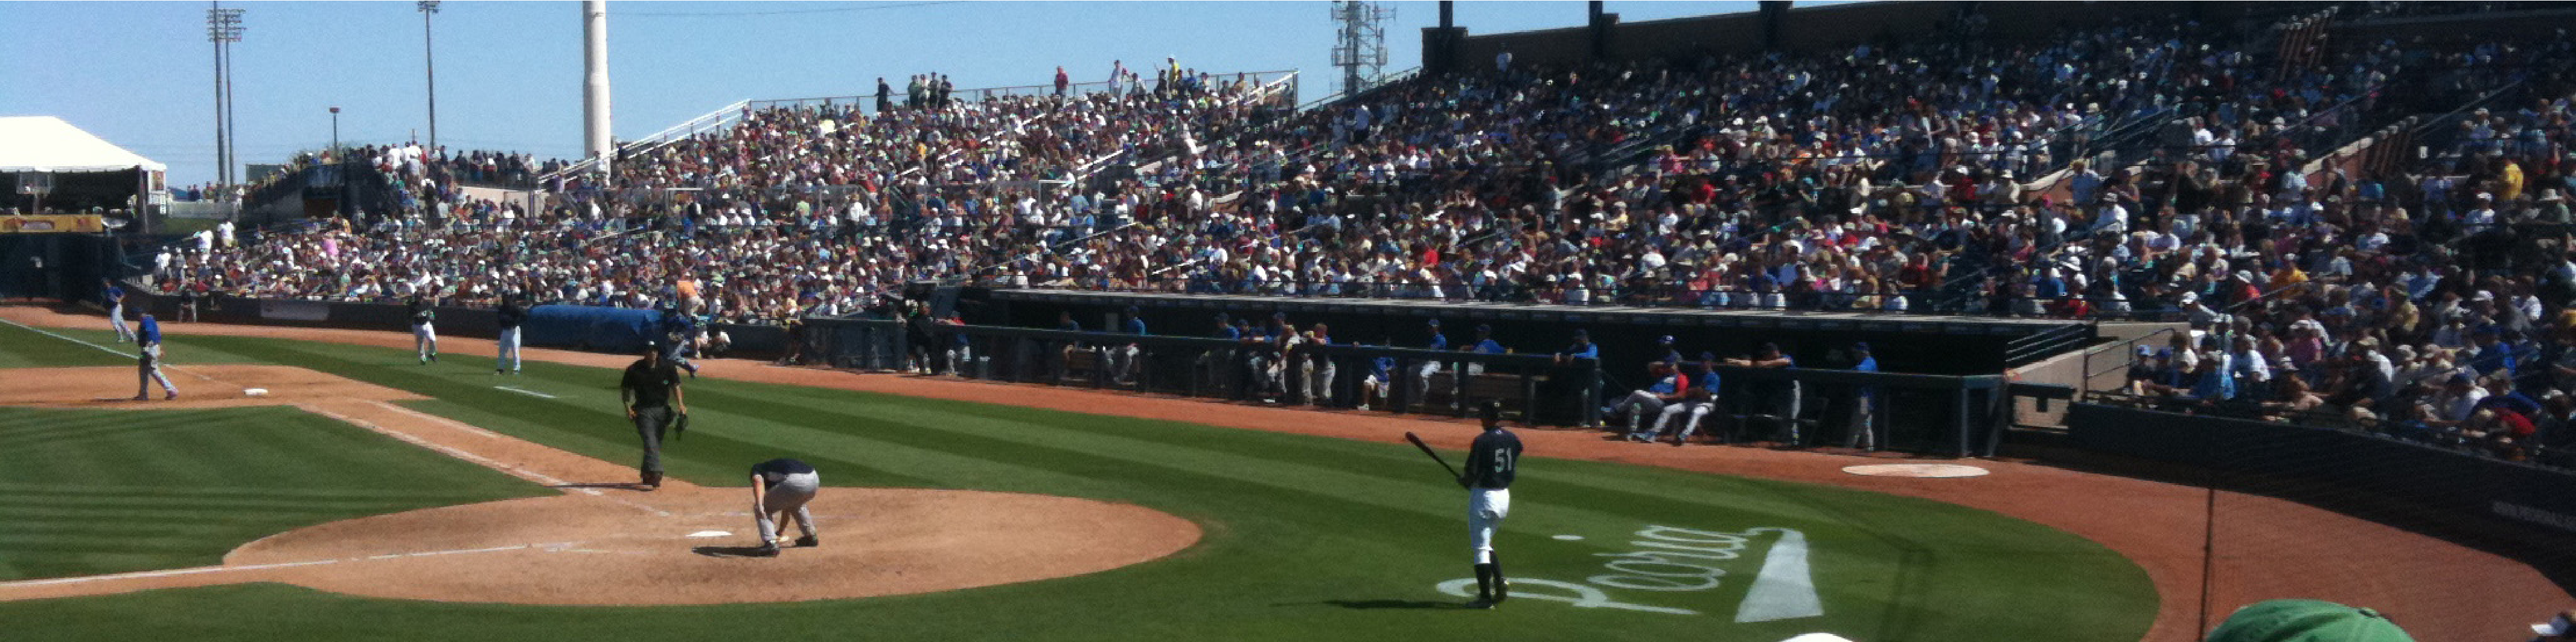
\includegraphics[width=\textwidth]{sampleteaser}
%  \caption{Seattle Mariners at Spring Training, 2010.}
%  \Description{Enjoying the baseball game from the third-base
%  seats. Ichiro Suzuki preparing to bat.}
%  \label{fig:teaser}
%\end{teaserfigure}

%%
%% This command processes the author and affiliation and title
%% information and builds the first part of the formatted document.
\maketitle

\section{Introduction}

Putting together learning materials for learners typically usually leads to some kind of
assessment as to whether or not the materials created are effective
\cite{ambrose2010learning, wilson2019teaching}.
However, the term ``effective'' is vague and ill-defined.
This leads to the creation of using learning objectives,
concrete tasks and goals learners are expected to meet at the end of teaching instruction.
The benefit of creating learning objectives is they are able to be measured and assessed.
These assessments can be used to gauge the efficacy of a lesson.

\subsection{Mental Models and Cognitive Load}

The Dreyfus model of skill acquisition describes how competency is acquired from
novies to expert practitioner
\cite{dreyfus1980five, bennerUsingDreyfusModel2004}.
Mental models are one way the bits of knowledge are connected together,
with novices having a lower number of nodes and connections compared to the
density of connections in expert practitioners.
Mental models can be represented physically as concept map diagrams
\cite{Koch2016, wilson2019teaching}.
Learner's existing mental models represent existing knowledge in their long-term memory (LTM).
When teaching new concepts,
more nodes are added to the model model of the learner.
Before these new nodes can be solidified, they are stored in working memory (WM)
before transitioning into short-term memory (STM) and LTM.
\cite{Koch2016, hermansProgrammerBrain2021, wilson2019teaching}.

Understanding how memory works in the context of teaching
helps determine the amount of information presented.
For novices, because they lack the necessary density of connections and knowledge (LTM),
each new bit of information (STM) requires more processing power (WM).
Concept maps help plan how much working memory and short-term memory learners are using during a lesson,
and lessons should follow George Miller's $7\pm2$ rule of how many items people can store in their STM
\cite{miller1956magical}.
More recent research suggests that the STM is even smaller, two (2) to six (6) items
\cite{hermansProgrammerBrain2021},
or $4\pm1$ \cite{didauWhatEveryTeacher2016}.

\subsection{Assessments and Learning Objectives}

One of the steps in planning out a lesson using a backward design is creating the assessment questions.
Assessments come in 2 main forms: formative and summative.
Formative assessments are the exercises students do during the course of instruction
in order to monitor student learning
\cite{universityFormativeVsSummative, wilson2019teaching}.
They can interweave within a single instructional period (e.g., clicker type questions),
or between instructional periods (e.g., quizzes, homework assignments).
The main goal of formative assessments is to keep the learner engaged with the learning materials,
and for both the instructor and learner to gauge learning by identifying areas that have not been grasped by the
learner or areas that need more review.
Formative assessments are typically low-stakes and given out frequently so the instructor
can get an accurate gauge of how well the learners are doing
\cite{universityFormativeVsSummative, wilson2019teaching}.

In contrast, summative assessments are given at the end of an instructional period
to evaluate student learning
\cite{universityFormativeVsSummative, wilson2019teaching}.
These types of assessments are the ``summation'' of multiple topics and can be given
during a course of instruction (e.g., midterm exam)
or towards the end of a course of instruction (e.g., final exam, thesis paper).
Summative assessments are typically high-stakes and
are used to gauge whether or not learners met learning objectives or
prerequisite knowledge for subsequent courses or lessons
\cite{universityFormativeVsSummative, wilson2019teaching}.

When designing assessment questions, there are many different ways questions can be formatted.
Two that we explore the use of faded examples (i.e., fill in the blanks)
and their performance to a ``blank'' problem.
Faded examples are code questions with the solution partially removed (i.e., components faded out)
and require the user to fill in the missing components to solve the question.
This type of question focuses the learner on what is important about the question,
and allows the instructor to lower the cognitive load of a question by filling in
extraneous parts of the solution (e.g., function input parameters).
This study then looks at time-to-completion and solution correctness
when faded examples are compared to a regular question without pre-populated solutions,
with and without an auto-code grader that can parse out the code submission and
tell the student where
exactly in their submission does not match the solution,
instead of a binary correct-incorrect response.

\section{Methods}


Two (2) separate workshops were run.
All data and access to the exercises were conducted through Qualtrics.
Participants consented at the start of the study and provided a unique user identifier
(Supplemental \ref{sse:assessment-study}).
The identifier was used to randomize participants into one (1) of four (4) treatment arms.
All exercise questions were created using R \code{learnr} documents,
depending on the treatment arm, each exercise question was paired with or without
the \code{gradethis} auto code grader.

The workshop began with a pre-workshop exercise.
During the workshop, three (3) 3 topics were covered and a short exercise (i.e., formative assessment)
was presented at the end of each topic.
The exercises fall into one of the four treatment arms for how the exercise is presented.
The end of the main workshop content was followed up with a final summative assessment question.
The amount of time to access the exercise and submit solution code was collected
along with user identifier and code solution for all of the coding questions.
Time to completion and code solutions were analysed and graded with a rubric.

\subsection{Treatment Arms}

The study created 4 treatment arms to look at exercise type and whether or not an auto-grader for
real-time feedback helps with student learning:
(1) blank exercise + no auto grader,
(2) faded example + no auto grader,
(3) blank exercise + auto grader, and
(4) faded example + auto grader.

Blank exercises only contained the programming question and a space for participants to type and execute R code.
Faded exercises contained the same programming question,
but the space participants would type and execute R code would be pre-populated with the solution with
function calls and arguments blanked out with a \code{\_\_}
(e.g., if the solution was \code{read\_csv(``mydata.csv'')},
the faded example would look like \code{\_\_(\_\_)} ).

\subsection{Randomization}

Block randomization was used to randomize participants.
A randomization list was pre-generated with a
seed of 42, 4 treatment groups, block size of 8, and no stratification factors
\cite{sealedenvelopeltdCreateBlockedRandomisation2021}.
The second workshop re-generated the randomization list to balance out the group responses.
Allocation ratios were adjusted for the second workshop due to varying amounts of participation
and attrition after initial randomization from the workshop sign-in from the first workshop.
Group 3 had 0 responses from the first workshop.
The second randomization doubled the weight for Group 3,
effectively creating a 5th treatment group, and used a block size of 10 for randomization.
Participants were asked to sign-in at the start of the workshop,
and their unique identifier was used for randomization.

\subsection{Workshop Content}

The workshop delivered was  the ``Tidy Data'' portion of the ds4biomed (ds4biomed.tech) materials. %todo add citation.
This lesson starts with the understanding that learners know about
(1) spreadsheets,
(2) loading data into R,
(3) subsetting columns and rows of data,
(4) calculating grouped aggregate summary statistics.
The workshop for this study started off with a pre-workshop survey that served as an assessment of
prerequisite knowledge.
The content workshop remained exactly the same as previous workshops and studies
that covered tidy data principles.
The only major change was forcing time for the formative and summative assessment questions.
Participants were given 5 minutes to work on the pre-workshop and formative assessment questions
and the solution was reviewed before continuing to the next topic.
15 minutes were allocated for the summative assessment question at the very end of the workshop.
The summative assessment question solution was provided after the workshop to fit within the
90-minute time limit for the workshop.

\subsection{Exercise Questions}

There was a total of 5 exercises presented to participants for this study:
(1) one pre-workshop exercise that asks participants to perform a small data pipeline task that they would
have been taught by now in the full 6-hour workshop version,
(2) three formative exercise questions, and
(3) one final summative assessment question.
Each exercise question had a space for the participant to enter and run the existing R code.
The exercise questions were written in R using the \code{learnr} package to create the documents,
and the \code{gradethis} package to grade the solutions and provide feedback results.
Workshop questions were deployed to \code{shinyapps.io}\footnote{https://www.shinyapps.io/}.
The links provided to the participants led them to the corresponding exercise across each of the treatment arms.

\subsubsection{Pre-workshop Exercise}

The pre-workshop exercise question is used as a baseline example since participants should
be able to accomplish these tasks by this point of the workshop.
The summative assessment example also uses concepts here during its data processing example.
Participants were asked the following question:

\begin{displayquote}
	
	Please write the code for the following pipeline steps:
	
	\begin{enumerate}
		\item Load the \code{tidyverse} and \code{readxl} libraries.
		\item Read in the Excel file located in:
		\code{"data/medicaldata\_tumorgrowth.xlsx"} into a variable \code{tumor}.
		\item Select the all the columns except \code{Grp},
		and filter the rows such that \code{Day} is \code{0} or \code{20}.
		Save this data subset into a variable \code{tumor\_subset}.
		\item We want to compare baseline tumor sizes (Day 0) with tumor sizes at Day 20 between each of the groups.
		Using \code{tumor\_subset},
		calculate the average tumor \code{Size} for each \code{Grp} and \code{Day}.
		\item Save \code{tumor\_subset} into a CSV file located in \code{"data/tumorsubset.csv"}.
	\end{enumerate}
	
\end{displayquote}

\subsubsection{Formative Assessment Exercise 1}

\begin{displayquote}
	Take a look at the \code{ebola} dataset.
	\begin{enumerate}
		\item Tidy the dataset such that you get the dataset below.
		\item You can use the \code{last\_col()} to select the last column of the dataset.
		\item Remember to drop missing values as the last step.
	\end{enumerate}
\end{displayquote}

\begin{figure}[htb]
    \centering
    \begin{subfigure}[h]{0.40\textwidth}
        \centering
        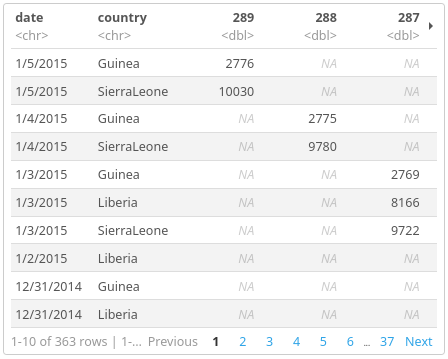
\includegraphics[scale=0.4]{figs/040-exercises/ex1-pre.png}
        \caption{Subcaption number one}
        \label{sfig:form_ass_ex_1_start}
    \end{subfigure}
    \begin{subfigure}[h]{0.40\textwidth}
        \centering
        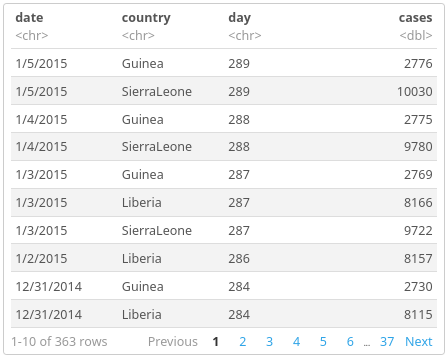
\includegraphics[scale=0.4]{figs/040-exercises/ex1-sol.png}
        \caption{Subcaption number two}
        \label{sfig:form_ass_ex_1_solution}
    \end{subfigure}

    \caption{Here is my main caption describing the relationship between the 4 subimages}
    \label{fig:main_figure}
\end{figure}


\subsubsection{Formative Assessment Exercise 2}
\begin{displayquote}
	
	This is a different version of the \code{ebola} dataset.
	
	\begin{enumerate}
		\item Tidy the dataset such that you get the dataset below
		\item Remember to drop missing values as the last step
	\end{enumerate}
	
\end{displayquote}

\begin{figure}[htb]
    \centering
    \begin{subfigure}[h]{0.40\textwidth}
        \centering
        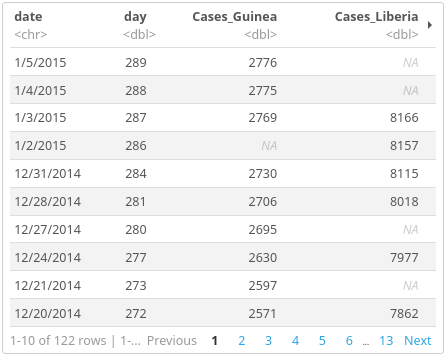
\includegraphics[scale=0.4]{figs/040-exercises/ex2-pre.png}
        \caption{Subcaption number one}
        \label{sfig:form_ass_ex_1_start}
    \end{subfigure}
    \begin{subfigure}[h]{0.40\textwidth}
        \centering
        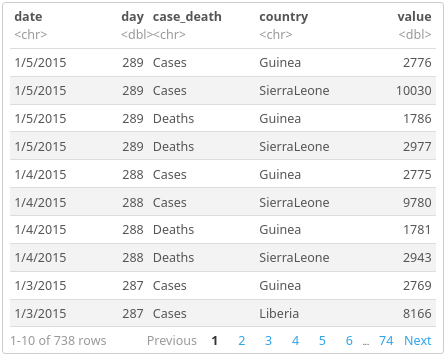
\includegraphics[scale=0.4]{figs/040-exercises/ex2-sol.png}
        \caption{Subcaption number two}
        \label{sfig:form_ass_ex_1_solution}
    \end{subfigure}

    \caption{Here is my main caption describing the relationship between the 4 subimages}
    \label{fig:main_figure}
\end{figure}

\subsubsection{Formative Assessment Exercise 3}

\begin{displayquote}
	
	This is a different version of the \code{ebola} dataset.
	
	\begin{enumerate}
		\item Tidy the dataset such that you get the dataset below
		\item Remember to drop missing values as the last step
	\end{enumerate}
	
\end{displayquote}

\begin{figure}[htb]
    \centering
    \begin{subfigure}[h]{0.40\textwidth}
        \centering
        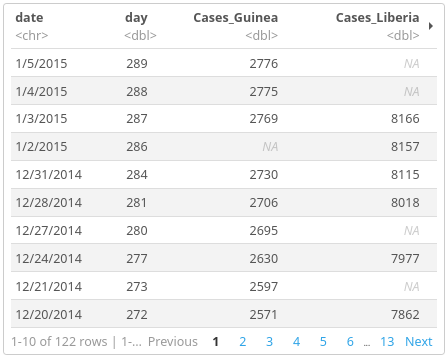
\includegraphics[scale=0.4]{figs/040-exercises/ex3-pre.png}
        \caption{Subcaption number one}
        \label{sfig:form_ass_ex_1_start}
    \end{subfigure}
    \begin{subfigure}[h]{0.40\textwidth}
        \centering
        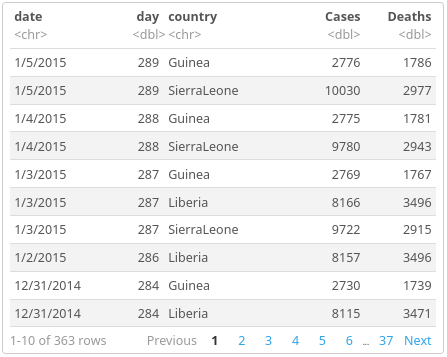
\includegraphics[scale=0.4]{figs/040-exercises/ex3-sol.png}
        \caption{Subcaption number two}
        \label{sfig:form_ass_ex_1_solution}
    \end{subfigure}

    \caption{Here is my main caption describing the relationship between the 4 subimages}
    \label{fig:main_figure}
\end{figure}

\subsubsection{Summative Assessment}

The summative assessment question is the same question from the post-workshop and long-term survey question
given to participants who participated in the full workshop sessions.
The question given in the previous studies did not ask participants to code up the solution,
rather it asked how confident participants are in their ability to complete a set of data tasks.
This study asks the participants to actually code up the results that will be graded.

\begin{displayquote}
	
	This is the cmv dataset you will load:
	
	\begin{enumerate}
		\item Use the \code{readxl} library to load the \code{"data/cmv.xlsx"} into a variable, \code{cmv}
		\item Filter the \code{cmv} dataset such that only $\text{age} > 65$ are remaining.
		Save this to a variable, \code{cmv\_subset}.
		\item Save the \code{cmv\_subset} variable to a csv file in \code{"data/cmv\_subset.csv"}.
	\end{enumerate}
	
	\begin{enumerate}
		\item Tidy the \code{cmv} dataset such that it looks like the clean dataset below.
		Save the tidy dataset into a variable, \code{cmv\_tidy}.
	\end{enumerate}
	
	\begin{enumerate}
		\item In the \code{cmv\_tidy} dataset, calculate the average age for each value of cmv.
	\end{enumerate}
	
\end{displayquote}

\subsection{Grading Rubric}

A grading rubric was created to score the participant-submitted code solutions.
A composite score for each exercise solution was created based on multiple factors.
1 point was awarded for each correct function call or similar function that achieves the same results.
Grading was done with the actual treatment group blinded to the grader,
scores were then combined with the rest of the full data for analysis.

\paragraph{Pre-Workshop Exercise}

7 points total.
Submission was graded on:
(1) loading library packages using the \code{library} function,
(2) loading data using the \code{read\_excel} function,
(3) subsetting columns using the \code{select} function,
(4) subsetting rows based on a condition using the \code{filter} function,
(5) aggregating summary statistics with the \code{group\_by} function,
(6) calculating the mean on grouped variables with the \code{summarize} function, and
(7) writing out results to an external file with the \code{read\_csv} function.


\paragraph{Exercise 1}

4 points total.
Submission was graded on:
(1) reshaping the dataset with the the \code{pivot\_longer} function,
(2) correctly selecting the columns for the \code{pivot\_longer} function,
(3) correctly specifying the new columns after the \code{pivot\_longer} function call, and
(4) dropping missing values with \code{drop\_na} function.

\paragraph{Exercise 2}

6 points total.
Submission was graded on:
(1) reshaping the dataset with the the \code{pivot\_longer} function,
(2) correctly selecting the columns for the \code{pivot\_longer} function,
(3) splitting column values with the the \code{separate} function,
(4) selecting the correct column to separate,
(5) using the correct separating delimiter, and
(6) ping missing values with \code{drop\_na} function.

\paragraph{Exercise 3}

3 points total.
Submission was graded on:
(1) reshaping the dataset with the the \code{pivot\_longer} function,
(2) reshaping the dataset with the the \code{pivot\_wider} function, and
(3) dropping missing values with \code{drop\_na} function.

\paragraph{Summative Assessment Exercise}

7 points total.
Submission was graded on:
(1) loading data using the \code{read\_excel} function,
(2) subsetting rows based on a condition using the \code{filter} function,
(3) saving the filtered dataset to a file with the \code{read\_csv} function,
(4) reshaping and tidying the dataset with the the \code{pivot\_longer} function,
(5) aggregating summary statistics with the \code{group\_by} function,
(6) calculating the mean on grouped variables with the \code{summarize} function, and
(7) writing out results to an external file with the \code{read\_csv} function.

\subsection{Analysis}

Three (3) different sets of values were compared across each of the 4 treatment arms:
(1) continuous variable of exercise solution score based on the grading rubric,
(2) continuous variable of time to exercise completion, and
(3) binary variable of whether the solution submitted is correct.
The final results did not include the binary variable analysis due to sample size.

Non-code solutions were dropped (e.g., pasted in a URL instead of solution code)
and not graded, as opposed to a score of 0.
Participants who attended both workshop sessions had their responses removed from the repeat session.
Participants who attempted the exercise questions more than once had the higher score kept for analysis,
in the event of a score tie, the first submission was used for analysis,
and other responses were dropped.

The R programming language and various supporting packages were used for analysis
\cite{allaireRmarkdownDynamicDocuments2021a, chenVennDiagramGenerateHighresolution2021, dahlXtableExportTables2019a, firkeJanitorSimpleTools2021a, ginnQualtRicsDownloadQualtrics2021b, grolemundDatesTimesMade2011, henryPurrrFunctionalProgramming2020a, henryTidyselectSelectSet2021a, hesterFsCrossplatformFile2021a, hesterGlueInterpretedString2021a, mullerHereSimplerWay2020a, mullerTibbleSimpleData2021a, oomsJsonlitePackagePractical2014a, oomsWritexlExportData2021a, wickhamDplyrGrammarData2021a, wickhamGgplot2ElegantGraphics2016a, wickhamReadrReadRectangular2021a, wickhamReadxlReadExcel2019, wickhamRvestEasilyHarvest2021a, wickhamStringrSimpleConsistent2019a, wickhamTidyrTidyMessy2021a, wickhamWelcomeTidyverse2019a, xieDynamicDocumentsKnitr2015a, xieKnitrComprehensiveTool2014a, xieKnitrGeneralpurposePackage2021a, xieMarkdownCookbook2020a, xieMarkdownDefinitiveGuide2018a}.


\section{Results}

The interpretations of the results from this study are limited due to attrition and low response rates.
The results are presented as preliminary data.
Due to the low sample size, treating the final summative assessment question as a binary variable of
correctness was not performed.
In general, none of the results had any statistical significance.

\subsection{Participants and Randomization}

Two (2) workshop sessions that covered the same materials and exercise content were given.
There were a total of 92 registrants (43 for session 1, and 49 for session 2)
and 44 workshop attendees (25 for session 1, and 19 for session 2).
30 participants were randomized across 4 arms
(Group 1: 8, Group 2: 7, Group 3: 8, Group 4: 7).

One (1) participant attended both workshops;
Any data from the second workshop was dropped from analysis.
One (1) participant attempted a question twice,
since the graded scores were the same for both attempts,
the first submission was kept for analysis.
One (1) code solution appeared to be code for a different question and was not scored and counted in the analysis.
A total of 16 randomized participants submitted at least 1 of the 5 exercises for analysis:
1 participant only took 1 exercise,
5 participants took 2 of the exercises,
2 participants took 3 of the exercises,
4 participants took 4 of the exercises, and
4 participants took all 5 exercises.
Table \ref{tab:exercise-treatment-response-counts} shows the number of
responses for each exercise and treatment group.

% from: 030-exercise_submission_descriptives.Rmd
% latex table generated in R 4.1.1 by xtable 1.8-4 package
% Thu Nov 25 23:34:34 2021
\begin{table}[ht]
	\centering
	\caption[Number of responses by group and exercise]
	{Number of code submissions for each group and exercise.
		There were a total of 16 randomized participants submitted at least one (1) of the five (5) exercises for analysis.
		The values listed in the \code{Total} column are the exercise response counts,
		and the values listed in the \code{sum} column are the group counts.
		The columns represent the
		treatment group,
		exercise 1 (ex1), exercise 2 (ex2), exercise 3 (ex3),
		pre-workshop exercise (pre), and
		post-workshop summative assessment (sum).
	}
	\begin{tabular}{rlrrrrr}
		\hline
		& treatment & ex1 & ex2 & ex3 & pre & sum \\
		\hline
		1 & Group 1 &   1 &   3 &   3 &   4 &   4 \\
		2 & Group 2 &   3 &   4 &   2 &   3 &   2 \\
		3 & Group 3 &   1 &   1 &   1 &   2 &   1 \\
		4 & Group 4 &   5 &   4 &   3 &   3 &   3 \\
		5 & Total &  10 &  12 &   9 &  12 &  10 \\
		\hline
	\end{tabular}
	\label{tab:exercise-treatment-response-counts}
\end{table}

\subsection{Exercise Scores}

The pre-workshop exercise was given out as a means to cover pre-requisite knowledge for the
summative assessment question.
Otherwise, the summative assessment would be no different from any of the other exercise
questions.
Since the summative assessment exercise relied on knowledge that was covered in the
pre-workshop exercise,
the 5 participants who received a full score of 7 in the pre-workshop exercise were analysed first.
Participants who scored well on the pre-workshop exercise also did well in all the other exercises
(Figure \ref{fig:exercise-scores-pre100}).
The 1 participant in Group 4 scored less than 50\% in the summative assessment question.
Figure \ref{fig:exercise-scores-separate-treatements} shows the percentage scores across each
of the exercises and treatment group.

\begin{figure}[!hbtp]
	\centering
	\includegraphics[width=0.9\textwidth]{figs/040-exercises/score\_prop-ex-treatment-facet_pre.png}
	\caption[Exercise scores of full scores and non full scores in pre-workshop exercise by treatment]
	{Distribution of scores for each treatment group across each exercise of
		respondents who received and did not receive a full score in the pre-workshop exercise.
		Participants who scored well on the pre-workshop exercise also did well in all the other exercises.
		The 1 participant in Group 4 scored less than 50\% in the summative assessment question.
	}
	\label{fig:exercise-scores-pre100}
\end{figure}

\begin{figure}[!hbtp]
	\centering
	\includegraphics[width=0.9\textwidth]{figs/040-exercises/score\_prop-ex-treatment-no\_facet.png.png}
	\caption[Graded Exercise Scores by treatment groups]
	{Distribution of exercise scores.
		Each participant's code submission was graded on a rubric.
		Scores are reported as a percentage because each exercise has a different total score.
		Score distributions were separate by whether or not a participant had a full score
		in the pre-workshop exercise (pre),
		since components of that are also used in the summative assessment question (sum).
		The other 3 exercises (ex1, ex2, ex3) were giving during the workshop
		as formative assessment questions.
		Results are also compared across 4 treatment groups:
		(1) Group 1: blank example with no auto code grader,
		(2) Group 2: faded example with no auto code grader,
		(3) Group 3: blank example with an auto code grader, and
		(4) Group 4: faded example with an auto code grader.
		Group 1 is the control group, and Group 4 is the main treatment of interest.
		
		The low sample size in each of the groups makes it difficult to make definitive conclusions.
		The data currently shows that participants who were able to get a full score
		in the pre-workshop exercise tend to also do well on the remaining exercise questions
		(Figure \ref{fig:exercise-scores-pre100}).
		More variation between exercises exists with participants who did not receive a full score
		in the pre-workshop exercise.
	}
	\label{fig:exercise-scores-separate-treatements}
\end{figure}

Some of the code solutions suggested that not every participant used the feature to execute their
code before submission.
Since we were unable to confirm if the autograder was used in these exercise treatment groups,
a separate analysis was performed that ignored the autograder,
so treatment groups 1 and 3 were combined together and treatment groups 2 and 4 were combined together
(Figure \ref{fig:exercise-scores-combined-treatments}).
These preliminary results seem to suggest that faded examples do not affect code results during the formative
assessments, but hinder results in the summative assessment question.
These differences disappear when pre-workshop exercise performance is taken into account
(Figure \ref{fig:exercise-scores-combined-groups-pre100}).

\begin{figure}[!hbtp]
	\centering
	\includegraphics[width=0.9\textwidth]{figs/040-exercises/score\_prop-ex-treatment-no\_facet-combine\_treatments.png}
	\caption[Graded Exercise Scores with combined treatment groups]
	{Distribution of exercise scores with the treatment groups combined by
		blank exercises (Groups 1 and 3) and faded examples (Groups 2 and 4).
		These groups were collapsed together since there was no way to track whether or not
		participants used the auto code grader.
		Preliminary results show that the faded examples do not differ from non-faded examples during
		the formative assessment questions,
		but the groups that used faded examples performed worse than those who were not given a faded example
		during the summative assessment question when all groups were provided an empty text field for the solution.
	}
	\label{fig:exercise-scores-combined-treatments}
\end{figure}

\begin{figure}[!hbtp]
	\centering
	\includegraphics[width=0.9\textwidth]{figs/040-exercises/score\_prop-ex-treatment-facet\_pre-combine\_treatments.png}
	\caption[Exercise scores of full scores and non full scores in pre-workshop exercise by combined treatment]
	{Distribution of scores for combined treatment groups across each exercise of
		respondents who received and did not receive a full score in the pre-workshop exercise.
		Participants who scored well on the pre-workshop exercise also did well in all the other exercises.
		The 1 participant in Group 4 scored less than 50\% in the summative assessment question.
	}
	\label{fig:exercise-scores-combined-groups-pre100}
\end{figure}

\subsection{Time to Complete}

Next, we wanted to see if there were any differences between types of exercises and amount of time to complete an exercise.
Faded examples provide a skeleton of the code for learners to fill-in instead of writing all of the code from scratch.
There did not seem to be any difference between time to exercise completion between the non-faded groups with the
faded example groups.
However these results suggest more about the amount of time learners needed to work on exercises.

\begin{figure}[!hbtp]
	\centering
	\includegraphics[width=0.9\textwidth]{figs/040-exercises/time\_to\_complete-ex-treatment-no\_facet-combine\_treatments.png}
	\caption[Time to complete exercises with combined treatment groups]
	{Distribution of time to complete exercises between treatment groups combined by
		blank exercises (Groups 1 and 3) and faded examples (Groups 2 and 4).
		These groups were collapsed together since there was no way to track whether or not
		participants used the auto code grader.
	}
	\label{fig:time-to-complete-combined-treatments}
\end{figure}

\section{Discussion}


This was a pilot study looking at how different kinds of assessment questions
and how they can be used to refine workshop content in a backward design approach.
Some of the code submissions suggested that not all students utilized all parts of the
coding platform,
so the use of the auto-grader could not assumed it was used in treatment arms 3 and 4.
The analysis was run with all 4 treatment groups, and with just 2 groups comparing
the blank question with the faded question.
Even with the low sample size from the study,
there are still findings that are applicable to data science instructors.

\subsection{Formative Assessments Engage Students In Remote Workshops}

The workshops were given in an online setting via Zoom.
The observation from the instructor of the workshop was there was almost zero
interaction of any kind during the workshop.
The vast majority of chat messages came from the instructor posting the
relevant links for each part of the workshop.
Very few questions or discussions occur in the zoom chatting platform.
There were more participants who took the exercises during the workshop than
questions and comments in the Zoom meeting room chat.
However, a surprisingly high number of students accomplished the exercises.
The amount of attrition was less than expected,
especially when comparing it to attrition from workshop registration to workshop attendance.

This finding suggests that even without grades as an incentive,
participants who volunteering opted in to participate in the workshop
were engaged with the materials, even in an online zoom setting.

\subsection{Give Learners Time to Practice and Learn Asynchronously}

Results from Figure \ref{fig:time-to-complete-combined-treatments} suggest more about
how much more time it takes a novice learner to complete exercises compared to experts.
Learners almost took the full 5-minutes for the formative assessment questions and
almost the full 15-minutes for the summative assessment question.
Using a conservative estimate for the instructor to go over the formative assessment solutions,
learners take about 4-times as long to complete formative assessment questions,
and almost 10-time as long to complete the summative assessment question.

During 1-hour of instruction, this means about 15-minutes would be needed for formative assessments,
leaving about 45-minutes to complete the main teaching materials.
In a workshop setting over multiple hours or sessions, lessons can be balanced across other parts of the workshop.
However, in individual workshop settings, additional time for setup would need to be
considered for every lesson.

This suggests that curating additional worked-out examples as formative assessment questions
should to be provided to learners
for asynchronous supplemental learning outside the main instructional period.

\subsection{Conclusion}

Although this was a pilot study, the results were able to show how pre-requisite knowledge plays a
role in learning new skills.
This study also showed how much more time learners need on answering formative and summative assessment questions compared to what an instructor imagines.
Both of these findings translate to live teaching sessions where prior knowledge can affect the learner's ability to pick up new information,
and planning how much content can be covered during an instructional period.
This study did not have a treatment arm that did not use any formative assessment,
but the participation rates from this study did hint that having formative assessments did force learners to be actively engaged with
the materials.
Using faded examples can reduce the amount of time spent on formative assessment questions when compared with a blank question box,
but it is possible that faded examples reduce too much of the cognitive load for solving problem from scratch.
This finding suggests that multiple types of formative assessment question types should be used in practice to balance
teaching time, student engagement, and student cognitive load.


%\section{Acknowledgments}
%
%Identification of funding sources and other support, and thanks to
%individuals and groups that assisted in the research and the
%preparation of the work should be included in an acknowledgment
%section, which is placed just before the reference section in your
%document.
%
%This section has a special environment:
%\begin{verbatim}
%  \begin{acks}
%  ...
%  \end{acks}
%\end{verbatim}
%so that the information contained therein can be more easily collected
%during the article metadata extraction phase, and to ensure
%consistency in the spelling of the section heading.
%
%Authors should not prepare this section as a numbered or unnumbered {\verb|\section|}; please use the ``{\verb|acks|}'' environment.
%
%\section{Appendices}
%
%If your work needs an appendix, add it before the
%``\verb|\end{document}|'' command at the conclusion of your source
%document.
%
%Start the appendix with the ``\verb|appendix|'' command:
%\begin{verbatim}
%  \appendix
%\end{verbatim}
%and note that in the appendix, sections are lettered, not
%numbered. This document has two appendices, demonstrating the section
%and subsection identification method.
%
%\section{SIGCHI Extended Abstracts}
%
%The ``\verb|sigchi-a|'' template style (available only in \LaTeX\ and
%not in Word) produces a landscape-orientation formatted article, with
%a wide left margin. Three environments are available for use with the
%``\verb|sigchi-a|'' template style, and produce formatted output in
%the margin:
%\begin{itemize}
%\item {\verb|sidebar|}:  Place formatted text in the margin.
%\item {\verb|marginfigure|}: Place a figure in the margin.
%\item {\verb|margintable|}: Place a table in the margin.
%\end{itemize}

%%
%% The acknowledgments section is defined using the "acks" environment
%% (and NOT an unnumbered section). This ensures the proper
%% identification of the section in the article metadata, and the
%% consistent spelling of the heading.
%\begin{acks}
%To Robert, for the bagels and explaining CMYK and color spaces.
%\end{acks}

%%
%% The next two lines define the bibliography style to be used, and
%% the bibliography file.
\bibliographystyle{ACM-Reference-Format}
\bibliography{bib, rpkgs}

%%
%% If your work has an appendix, this is the place to put it.
\appendix

\section{Research Methods}

\subsection{Survey Questions}
\label{sse:assessment-study}

Participants were asked to create a unique identifier to track them throughout all studies without
having to capture any identifiable information.

The question they were asked was adapted from the same question used in The Carpentries
workshop feedback questions
\cite{jordanAnalysisCarpentriesLongTerm2017, jordanAnalysisCarpentriesLongTerm2018, jordanAnalysisCarpentriesLongTerm2020, jordanAnalysisSoftwareCarpentry2017, jordanAnalysisSoftwareData2018, jordanCarpentries2020Annual, jordanDataCarpentryAssessment2016}.
Below is a reproduction of the question presented to participants:

\begin{displayquote}
	Please create a unique identifier.
	This unique identifier will be used to link your survey responses but keep your personal information anonymous.
	
	To create an identifier type in:
	\begin{enumerate}
		\item Number of siblings (as numeric) +
		\item First two (2) letters of the city you were born in (lower-case) +
		\item First three (3) letters of your current street (lower-case).
	\end{enumerate}
	
	E.g., Sherlock Homes has \textbf{1} brother,
	was born in \textbf{Po}rsmoth,
	and lives on \textbf{Bac}ker street would have the ID: \textbf{1pobac}
\end{displayquote}

%\section{Online Resources}
%
%Nam id fermentum dui. Suspendisse sagittis tortor a nulla mollis, in
%pulvinar ex pretium. Sed interdum orci quis metus euismod, et sagittis
%enim maximus. Vestibulum gravida massa ut felis suscipit
%congue. Quisque mattis elit a risus ultrices commodo venenatis eget
%dui. Etiam sagittis eleifend elementum.
%
%Nam interdum magna at lectus dignissim, ac dignissim lorem
%rhoncus. Maecenas eu arcu ac neque placerat aliquam. Nunc pulvinar
%massa et mattis lacinia.

\end{document}
\endinput
%%
%% End of file `sample-acmsmall-conf.tex'.
